\addcontentsline{toc}{section}{Introduction}
\section*{Introduction}

Ce chapitre présente les résultats concrets obtenus à l'issue de la conception et du développement de la plateforme \textit{Numeris229}. Il s'ouvre sur une démonstration détaillée des différentes interfaces utilisateur développées avec Next.js 14 et Tailwind CSS, illustrant la navigation ergonomique entre la page d'accueil, l'explorateur du Code du Numérique, l'espace de consultation juridique conversationnelle et les écrans de gestion de compte. Ensuite, il expose la méthodologie d'évaluation mise en œuvre pour valider la robustesse de l'API REST, l'exactitude du traitement des articles de loi et la pertinence du pipeline RAG souverain à travers l'analyse des scores de similarité cosinus. Enfin, le chapitre dresse un bilan lucide des limites actuelles du prototype et formule les perspectives d'évolution envisagées pour son déploiement à l'échelle nationale.

% ─────────────────────────────────────────────────────────
\section{Présentation de la solution}
% ─────────────────────────────────────────────────────────

La plateforme \textit{Numeris229} est matérialisée par une application web moderne, responsive et souveraine, accessible depuis tout navigateur internet conventionnel sur ordinateur, tablette et smartphone. L'interface s'appuie sur une charte graphique institutionnelle et épurée combinant un vert émeraude profond (\texttt{\#065F46} / \texttt{emerald-800}), rappelant l'autorité et la légalité, un gris ardoise (\texttt{slate}) pour les textes et bordures, ainsi qu'une prise en charge native du thème sombre (\textit{Dark Mode}) et d'un basculement bilingue (Français / Anglais).

\subsection{Barre de navigation et page d'accueil}

La page d'accueil (figure~\ref{fig:accueil_hero}) constitue la porte d'entrée institutionnelle de la plateforme. Elle est coiffée d'une barre de navigation fixe (\textit{Navbar}) comprenant le logo officiel \textbf{Numeris229}, des liens d'accès direct vers les sections clés (\textbf{Explorateur}, \textbf{À propos}, \textbf{Domaines}, \textbf{Fonctionnalités}), un sélecteur de langue interactif (FR/EN), un commutateur de thème (clair/sombre) ainsi que les boutons d'authentification (\textbf{Connexion} et \textbf{Inscription}).

\medskip

\noindent\textbf{La section Hero :} Elle accueille l'usager avec un badge institutionnel mettant en exergue le cadre légal de référence~: \og Loi N° 2017-20 modifiée • République du Bénin \fg{}. Le titre principal proclame avec solennité la mission du service~: \og L'intelligence artificielle au service du Code du Numérique béninois \fg{}. Il est soutenu par une description valorisant la précision juridique et l'absence d'hallucination. Deux boutons d'appel à l'action immédiate guident l'usager~:
\begin{itemize}
    \item \textbf{Démarrer une consultation :} bouton principal plein vert émeraude invitant à interroger l'assistant conversationnel RAG ;
    \item \textbf{Explorer les textes :} bouton secondaire avec bordure fine permettant de parcourir directement le catalogue exhaustif des articles de loi.
\end{itemize}

En pied de zone hero, trois encarts synthétiques rappellent les piliers fondateurs~: la recherche documentaire sans hallucination, la simplicité d'accès pour tous les citoyens et le déploiement local garantissant la souveraineté des données.

\begin{figure}[H]
  \centering
  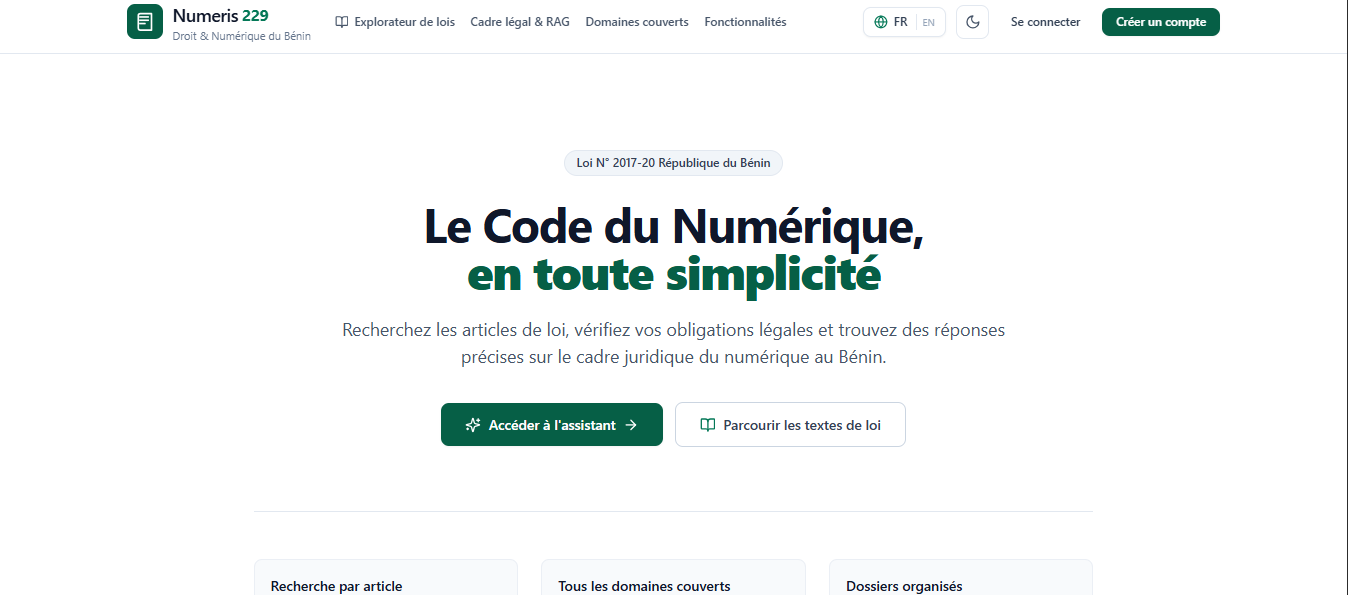
\includegraphics[width=\textwidth]{images/C3/1.png}
  \caption{Page d'accueil — Section d'en-tête et navigation de Numeris229}
  \label{fig:accueil_hero}
\end{figure}

\begin{figure}[H]
  \centering
  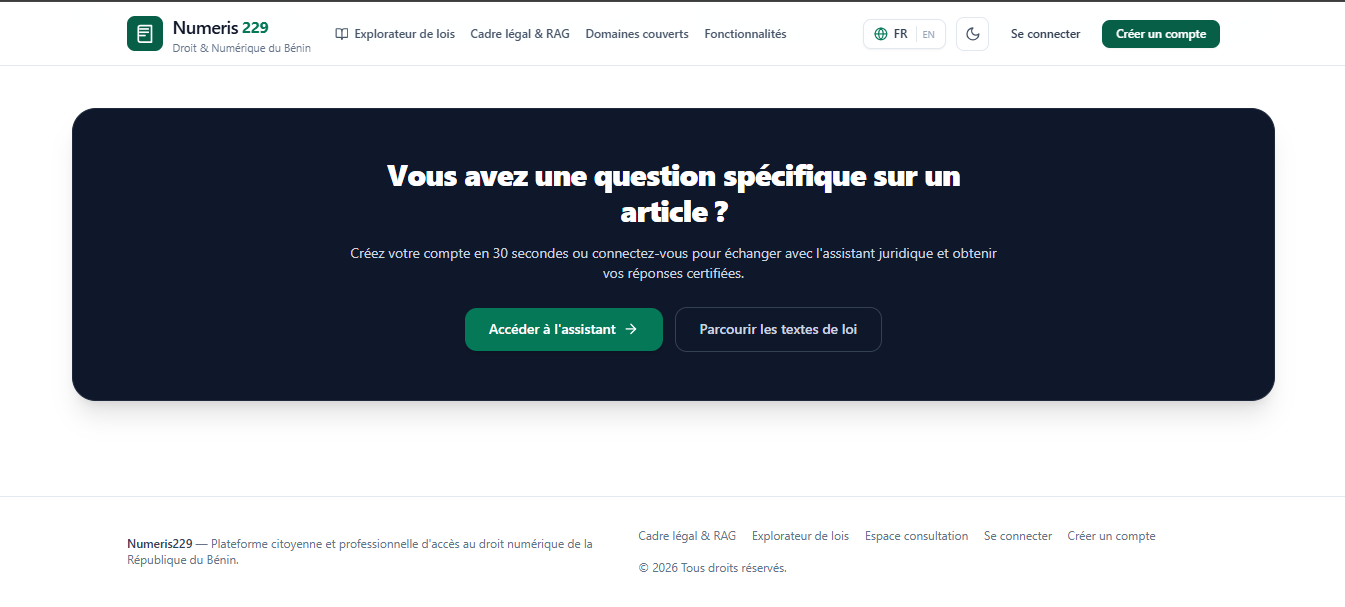
\includegraphics[width=\textwidth]{images/C3/6.png}
  \caption{Page d'accueil — Section de pied de page et navigation de Numeris229}
  \label{fig:accueil_hero}
\end{figure}

\medskip

\noindent\textbf{La section des atouts et fonctionnalités (figure~\ref{fig:accueil_features}) :} Agencée en une grille de six cartes interactives, cette section valorise les garanties techniques offertes par la solution~: citations obligatoires des articles officiels, recherche multimodale (par numéro ou thème), historique persistant des conversations, chiffrement fort des échanges, pipeline RAG haute performance et vulgarisation didactique du droit.

\begin{figure}[H]
  \centering
  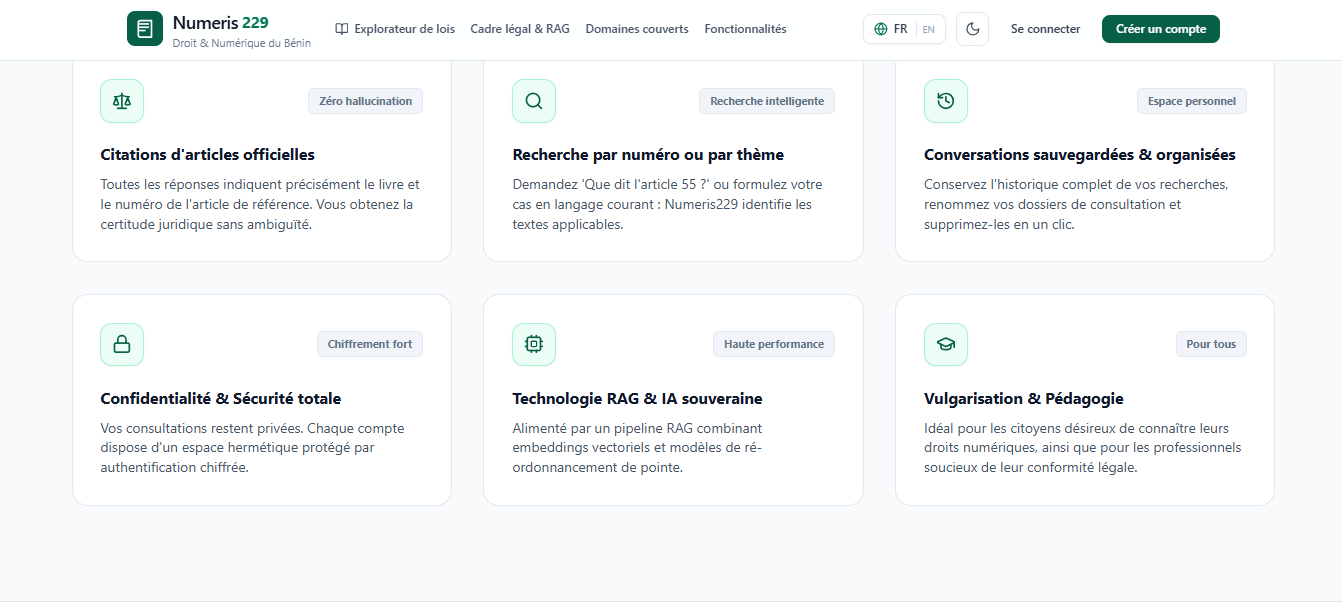
\includegraphics[width=\textwidth]{images/C3/3.png}
  \caption{Page d'accueil — Grille des fonctionnalités et garanties du système}
  \label{fig:accueil_features}
\end{figure}

\medskip

\noindent\textbf{La section des domaines juridiques couverts (figure~\ref{fig:accueil_domaines}) :} Cette section cartographie les quatre matières majeures régies par le Code du Numérique en République du Bénin, présentées sous forme de cartes structurées~:
\begin{enumerate}
    \item \textbf{Livre V — Protection des données à caractère personnel :} formalités préalables auprès de l'APDP, droits des personnes fichées, sanctions en cas de fuite de données ;
    \item \textbf{Livre VI — Cybercriminalité et répression pénale :} arnaques en ligne, diffamation par moyen électronique, usurpation d'identité et peines applicables ;
    \item \textbf{Livre III — Commerce et signature électronique :} validité probante des écrits électroniques, obligations contractuelles des sites marchands ;
    \item \textbf{Livre IV — Cybersécurité et confiance numérique :} obligations des opérateurs d'importance vitale, certifications de sécurité et rôle de l'ANSSI-Bénin.
\subsection{Espace personnel, sécurité et gestion du profil}

L'accès personnalisé à la plateforme est régi par un ensemble d'écrans dédiés à l'authentification et au respect de la vie privée.

\medskip


\end{enumerate}
Chaque carte est enrichie d'exemples concrets de questions cliquables permettant d'orienter immédiatement le citoyen vers une consultation juridique ciblée.

\begin{figure}[H]
  \centering
  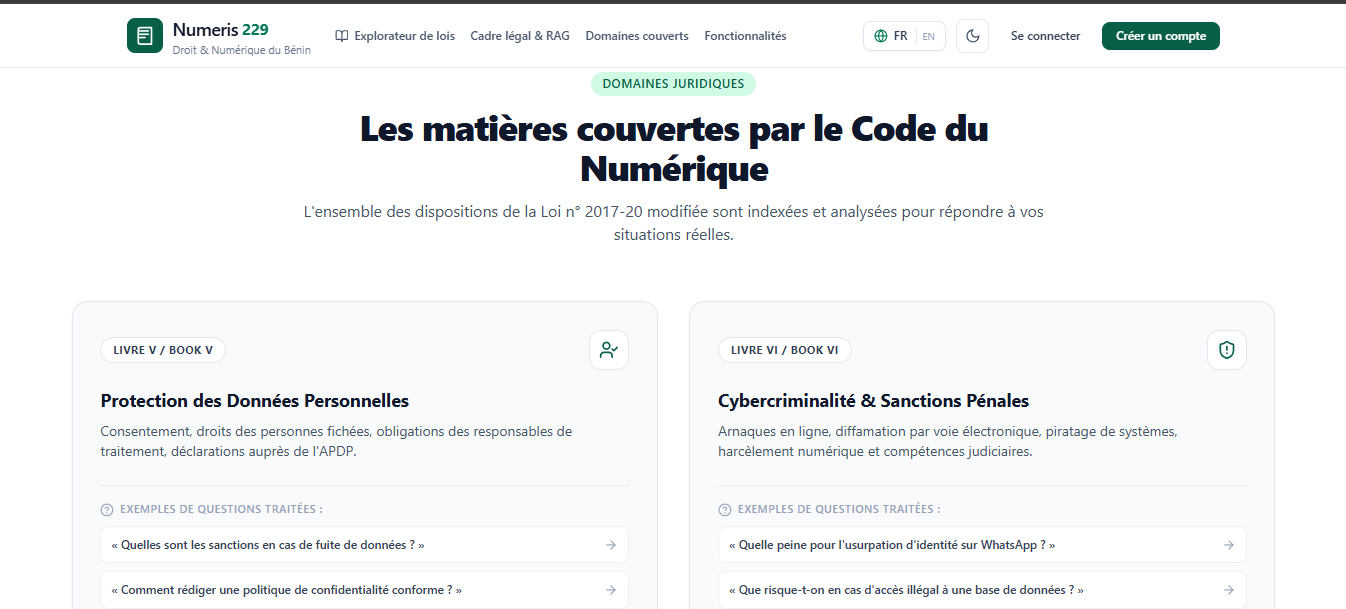
\includegraphics[width=\textwidth]{images/C3/4.png}
  \caption{Page d'accueil — Présentation des matières juridiques et cas d'usage 1}
  \label{fig:accueil_domaines}
\end{figure}

\begin{figure}[H]
  \centering
  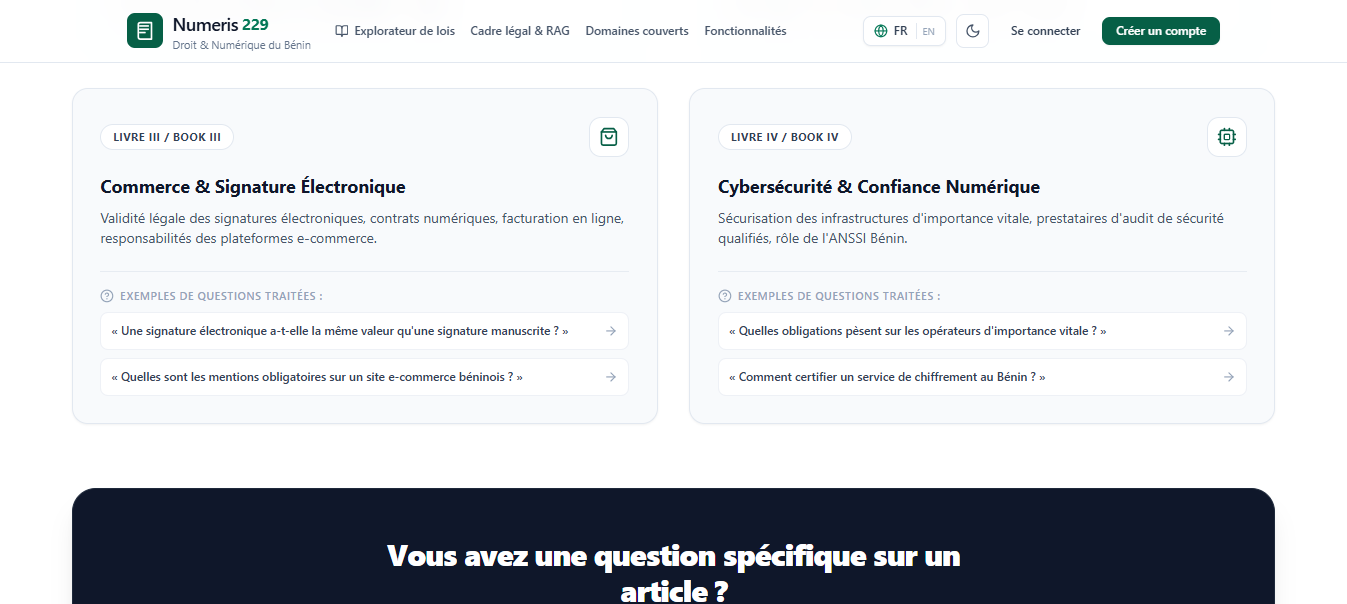
\includegraphics[width=\textwidth]{images/C3/5.png}
  \caption{Page d'accueil — Présentation des matières juridiques et cas d'usage 2}
  \label{fig:accueil_domaines}
\end{figure}

\noindent\textbf{Inscription et Connexion (figures~\ref{fig:auth_inscription} et~\ref{fig:auth_connexion}) :} Le formulaire d'inscription recueille les informations nécessaires à l'identification de l'usager (nom, prénoms, adresse électronique, numéro de téléphone, sexe, âge et profession) avec validation de la cohérence du mot de passe. L'écran de connexion valide les identifiants et délivre le jeton de session JWT. Un lien permet d'accéder au formulaire de réinitialisation de mot de passe par jeton temporaire en cas d'oubli.

\begin{figure}[H]
  \centering
  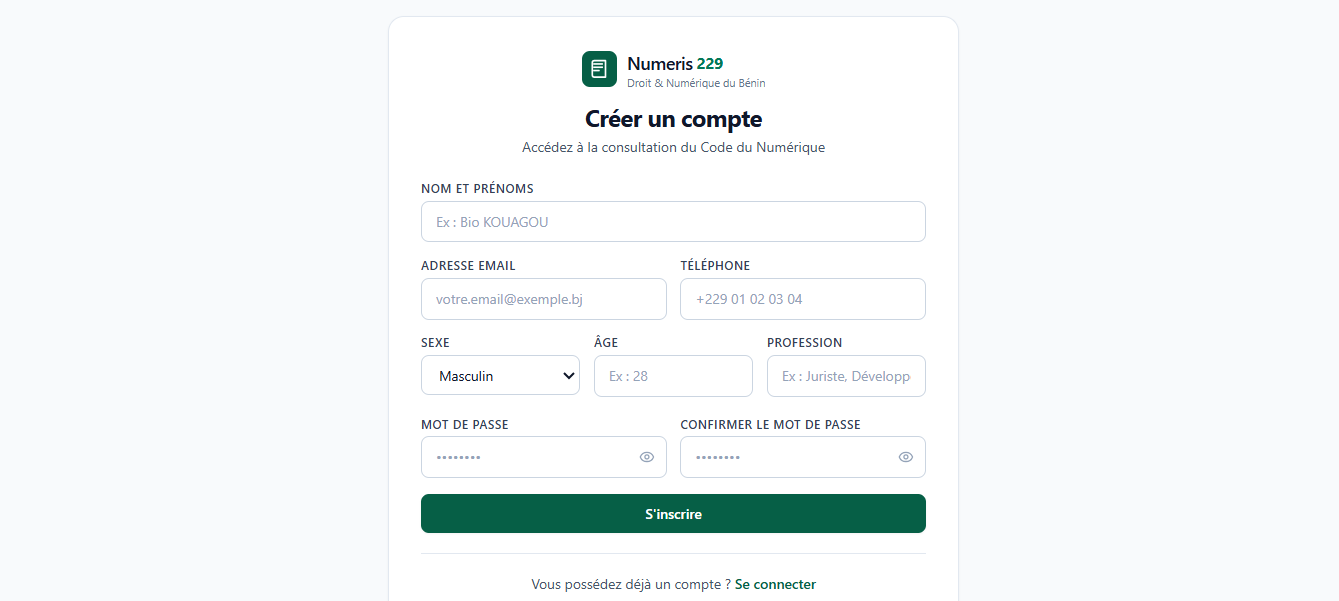
\includegraphics[width=0.75\textwidth]{images/C3/7.png}
  \caption{Interface d'inscription d'un nouvel utilisateur}
  \label{fig:auth_inscription}
\end{figure}

\begin{figure}[H]
  \centering
  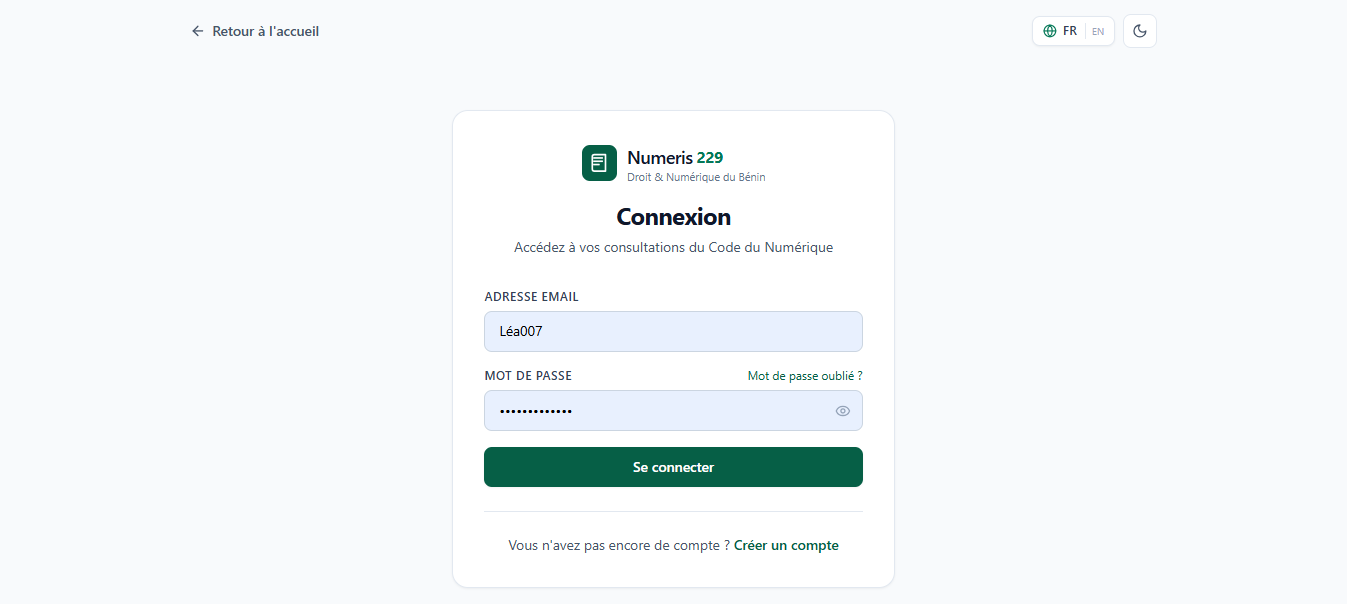
\includegraphics[width=0.7\textwidth]{images/C3/8.png}
  \caption{Interface de connexion et d'authentification sécurisée}
  \label{fig:auth_connexion}
\end{figure}

\medskip

\subsection{Explorateur du Code du Numérique}

La page de l'Explorateur (figure~\ref{fig:explorateur_liste}) offre un moteur d'exploration textuelle et thématique permettant de parcourir l'intégralité des dispositions législatives de la Loi N° 2017-20 modifiée par la Loi N° 2020-35.

\medskip

\noindent\textbf{La zone de filtrage et recherche en temps réel :} Placée sous l'en-tête institutionnel, elle intègre un champ de recherche réactif permettant de rechercher indifféremment par numéro d'article (ex.~: \og 55 \fg{}, \og 550 \fg{}) ou par mot-clé (ex.~: \og diffamation \fg{}, \og APDP \fg{}, \og consentement \fg{}). Ce champ est associé à une liste déroulante dynamique permettant de filtrer par Livre (Livre Préliminaire, Livres I à VI). Un compteur statistique informe instantanément l'utilisateur du volume exact d'articles correspondants aux critères actifs.

\medskip

\noindent\textbf{Les cartes d'articles et la pagination :} Les articles sont affichés sous forme de cartes aérées et paginées par tranche de 15~articles. Chaque carte expose en en-tête un badge vert \og Article X \fg{} ainsi que l'intitulé du Livre de rattachement. Le corps de la carte présente le titre officiel et les trois premières lignes du texte normatif. Au bas de chaque carte, trois actions sont proposées~:
\begin{itemize}
    \item \textbf{Lire le texte intégral :} ouvre un tiroir modal affichant l'intégralité de l'article sans coupure ;
    \item \textbf{Copier l'article :} enregistre la citation officielle complète dans le presse-papiers ;
    \item \textbf{Interroger l'IA :} redirige l'utilisateur vers l'espace de consultation conversationnelle en pré-remplissant automatiquement la question sur les implications de cet article précis.
\end{itemize}

\begin{figure}[H]
  \centering
  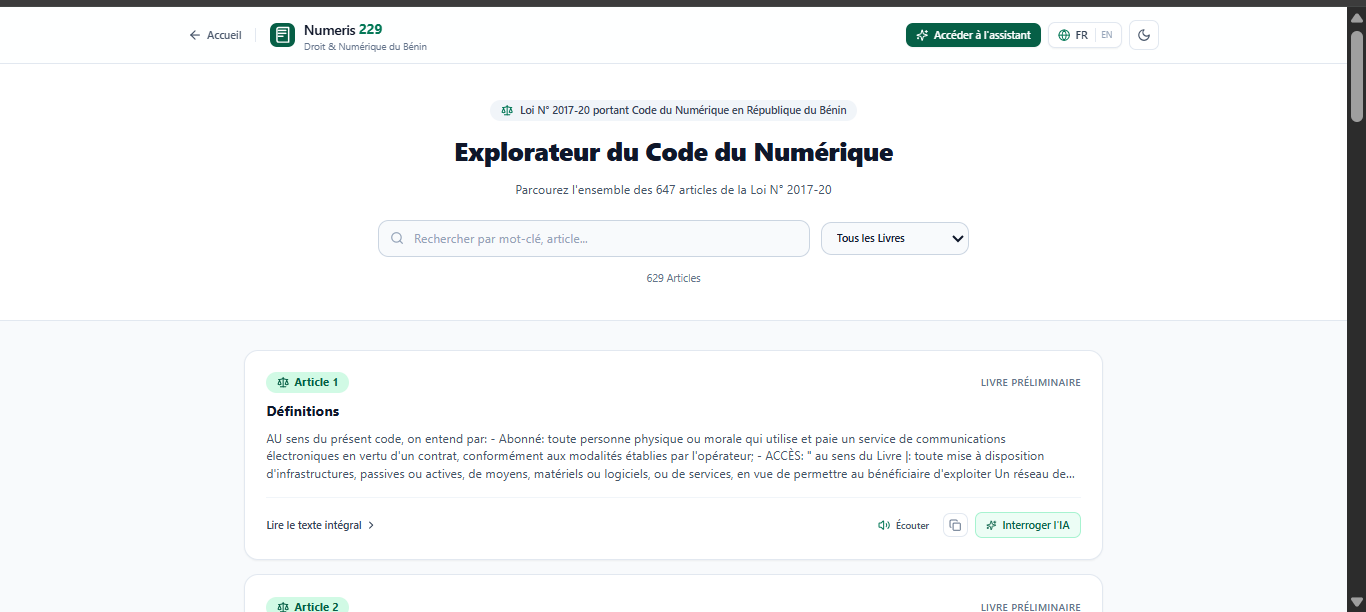
\includegraphics[width=\textwidth]{images/C3/13.png}
  \caption{Explorateur du Code du Numérique — Recherche dynamique et pagination}
  \label{fig:explorateur_liste}
\end{figure}

\medskip

\noindent\textbf{La fenêtre modale de lecture intégrale (figure~\ref{fig:explorateur_modal}) :} Conçue pour offrir un confort de lecture optimal, cette boîte de dialogue modale affiche la teneur intégrale de l'article sélectionné avec une typographie serif élégante. Lorsque l'article a fait l'objet d'une révision législative par la Loi N° 2020-35 du 06 janvier 2021, un encart d'avertissement ambré détaille la mention officielle de modification, prévenant toute ambiguïté juridique. Un bouton situé en bas de fenêtre permet d'interroger directement l'assistant IA sur cet extrait.

\begin{figure}[H]
  \centering
  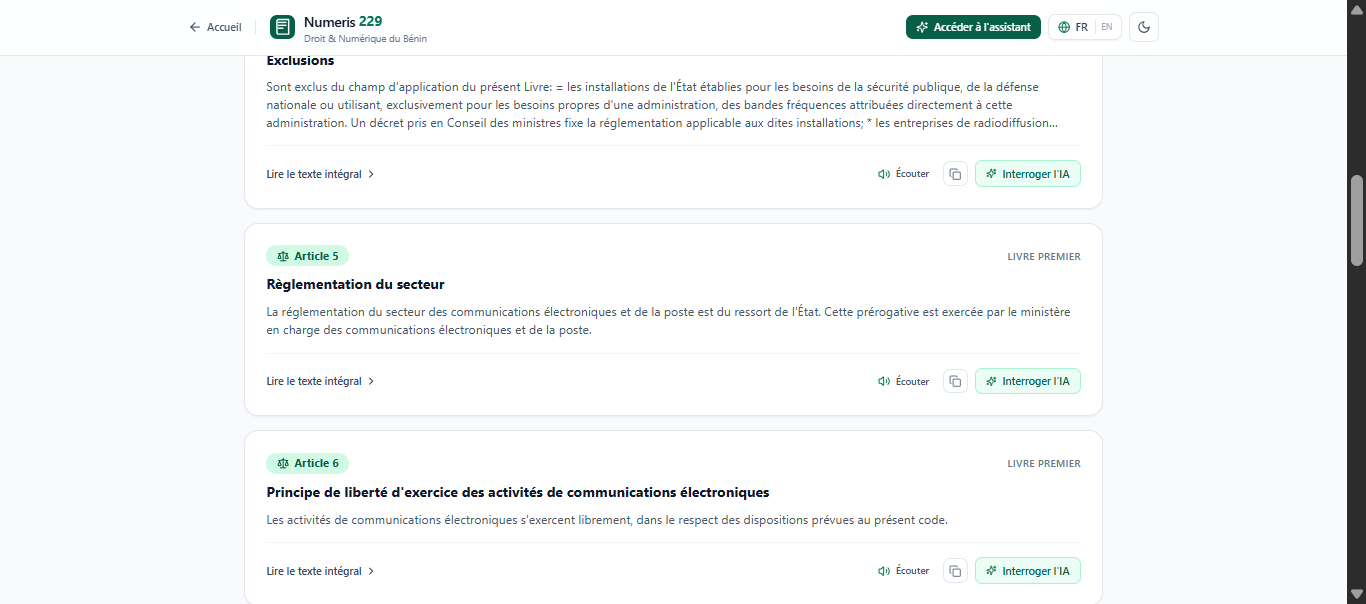
\includegraphics[width=0.85\textwidth]{images/C3/14.png}
  \caption{Explorateur — Fenêtre modale de consultation intégrale d'un article de loi}
  \label{fig:explorateur_modal}
\end{figure}

\begin{figure}[H]
  \centering
  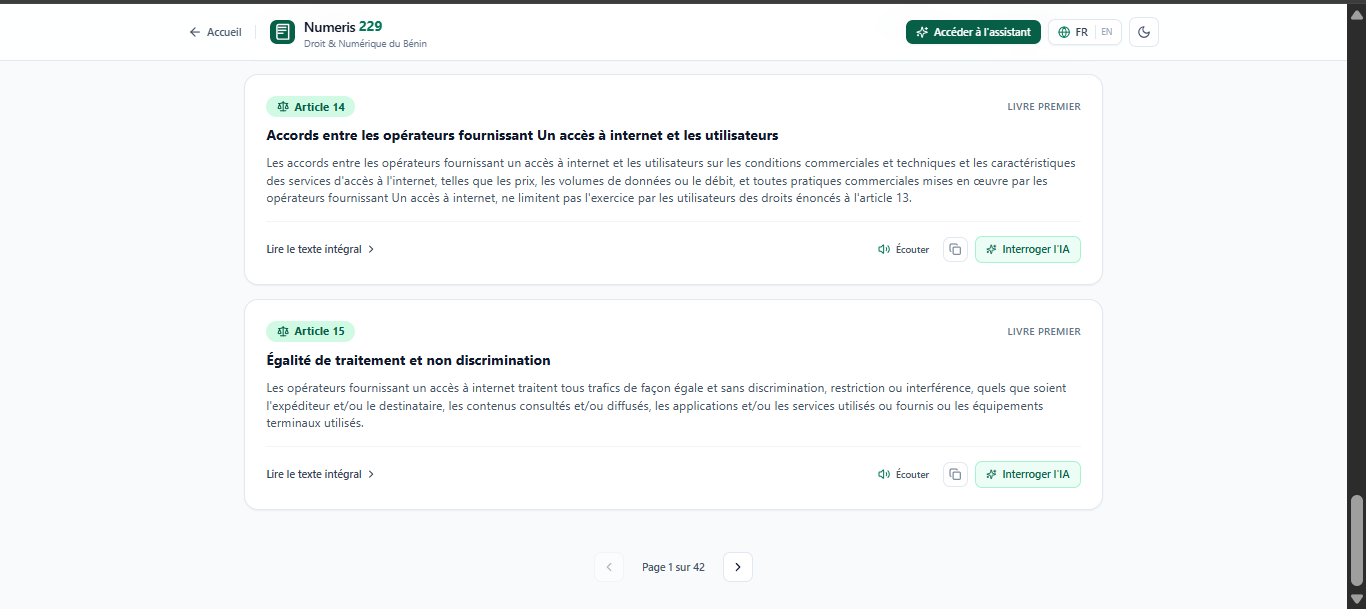
\includegraphics[width=0.85\textwidth]{images/C3/15.png}
  \caption{Explorateur — Fenêtre modale de consultation intégrale d'un article de loi}
  \label{fig:explorateur_modal}
\end{figure}

\subsection{Espace de consultation juridique conversationnelle (Chat RAG)}

L'espace de consultation (figures~\ref{fig:chat_vide} et~\ref{fig:chat_reponse}) matérialise l'interaction conversationnelle en langage naturel avec le modèle d'intelligence artificielle souverain.

\medskip

\noindent\textbf{Le volet latéral (Sidebar) :} Déployé sur la partie gauche, ce volet administre les sessions de consultation de l'utilisateur. Il propose un bouton d'action rapide \textbf{Nouvelle consultation} (\og + \fg{}) et dresse la liste antéchronologique des dossiers de discussion. Chaque entrée affiche un titre thématique généré automatiquement au premier échange, la date de création et des commandes contextuelles permettant de \textbf{renommer} le titre à la volée ou de \textbf{supprimer} définitivement la session conformément au droit à l'oubli. En pied de panneau, l'utilisateur retrouve un résumé de son identité, le commutateur de thème et le bouton de déconnexion.

\medskip

\noindent\textbf{L'écran d'accueil d'une consultation vierge (figure~\ref{fig:chat_vide}) :} En l'absence de message, la zone centrale arbore l'emblème de la justice (la balance), le titre de l'assistant et quatre suggestions thématiques cliquables conçues pour guider les premières interrogations du citoyen (peines pour diffamation, règles de collecte de données, valeur de la signature électronique, mentions légales e-commerce).

\begin{figure}[H]
  \centering
  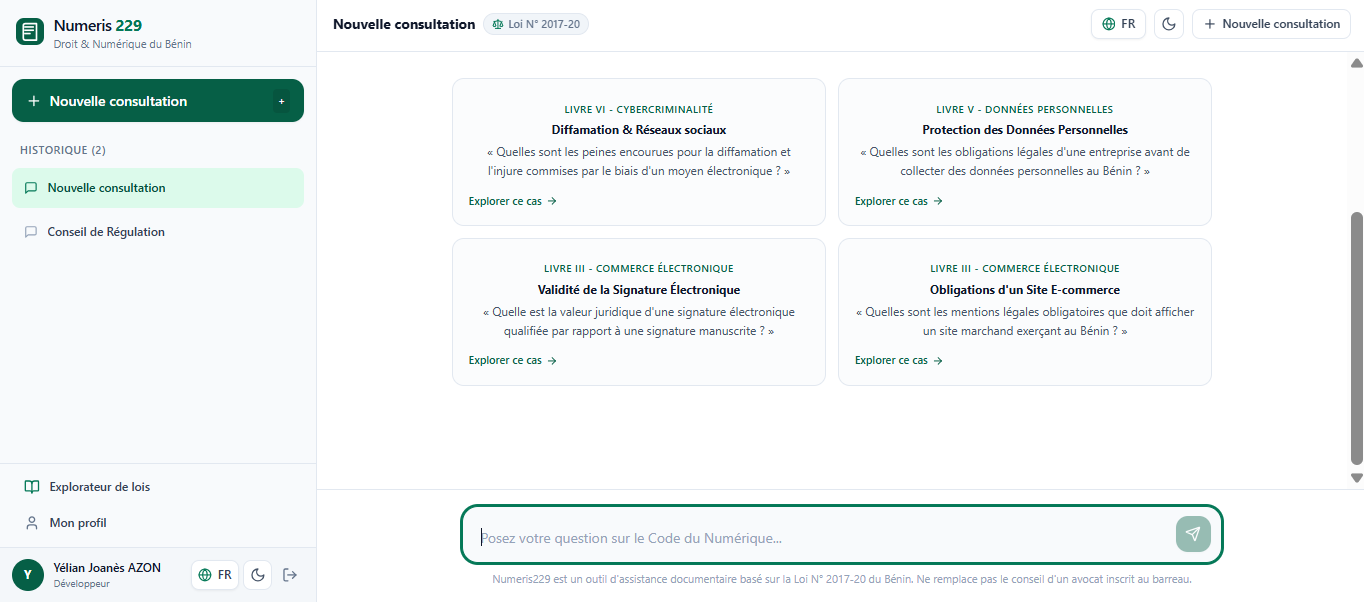
\includegraphics[width=\textwidth]{images/C3/10.png}
  \caption{Espace de consultation — Écran d'accueil et volet d'historique des sessions}
  \label{fig:chat_vide}
\end{figure}

\medskip

\noindent\textbf{Le fil de discussion et l'affichage des réponses sourcées (figure~\ref{fig:chat_reponse}) :} Lors d'une interaction, les messages de l'usager apparaissent alignés à droite dans des bulles vertes émeraude. Pendant le traitement par le pipeline RAG, un bandeau discret animé informe de l'analyse documentaire en cours (\og Recherche dans le Code du Numérique... \fg{}).

La réponse produite par l'assistant s'affiche à gauche dans une carte structurée. Elle comporte une barre d'en-tête mentionnant \og Numeris229 • Analyse juridique \fg{} ainsi qu'un bouton de copie rapide. Le texte de la réponse, rédigé en français formel et sans hallucination, commence systématiquement par citer l'article de loi de référence. 

En bas de carte, un composant accordéon interactif intitulé \textbf{\og X référence(s) juridique(s) citée(s) \fg{}} permet à l'usager de déplier les extraits textuels exacts du Code du Numérique retenus par le système, offrant une transparence et une vérifiabilité totales.

\begin{figure}[H]
  \centering
  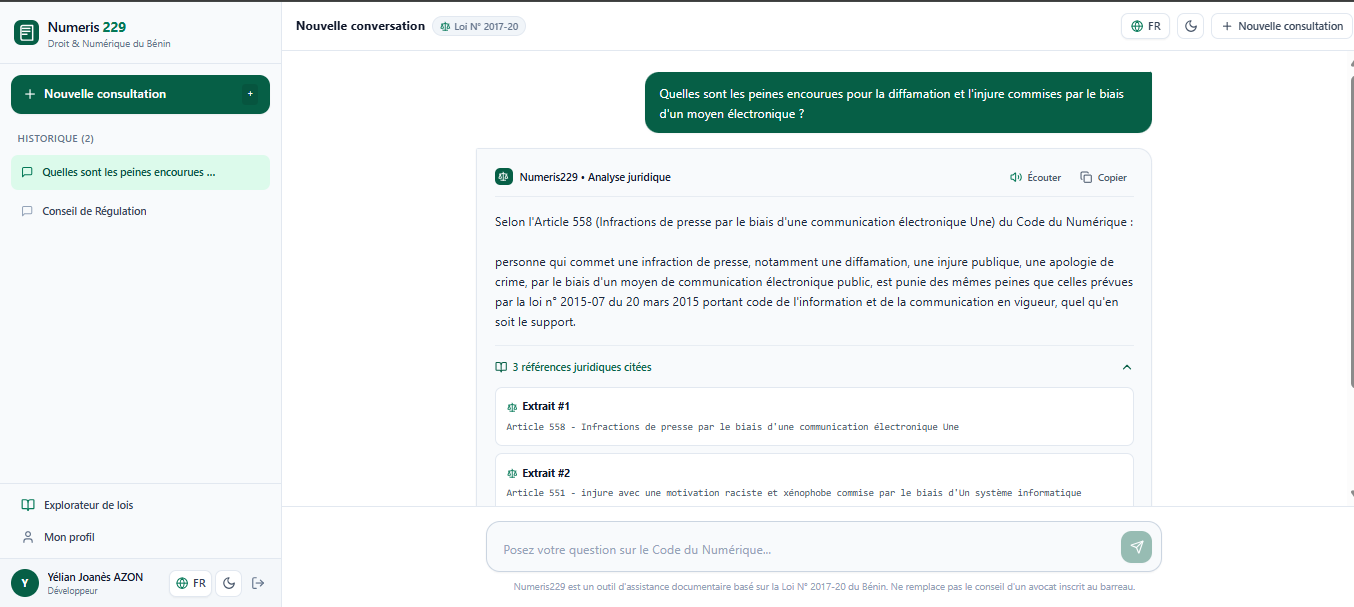
\includegraphics[width=\textwidth]{images/C3/11.png}
  \caption{Espace de consultation — Restitution d'une analyse juridique avec sources dépliables}
  \label{fig:chat_reponse}
\end{figure}

\begin{figure}[H]
  \centering
  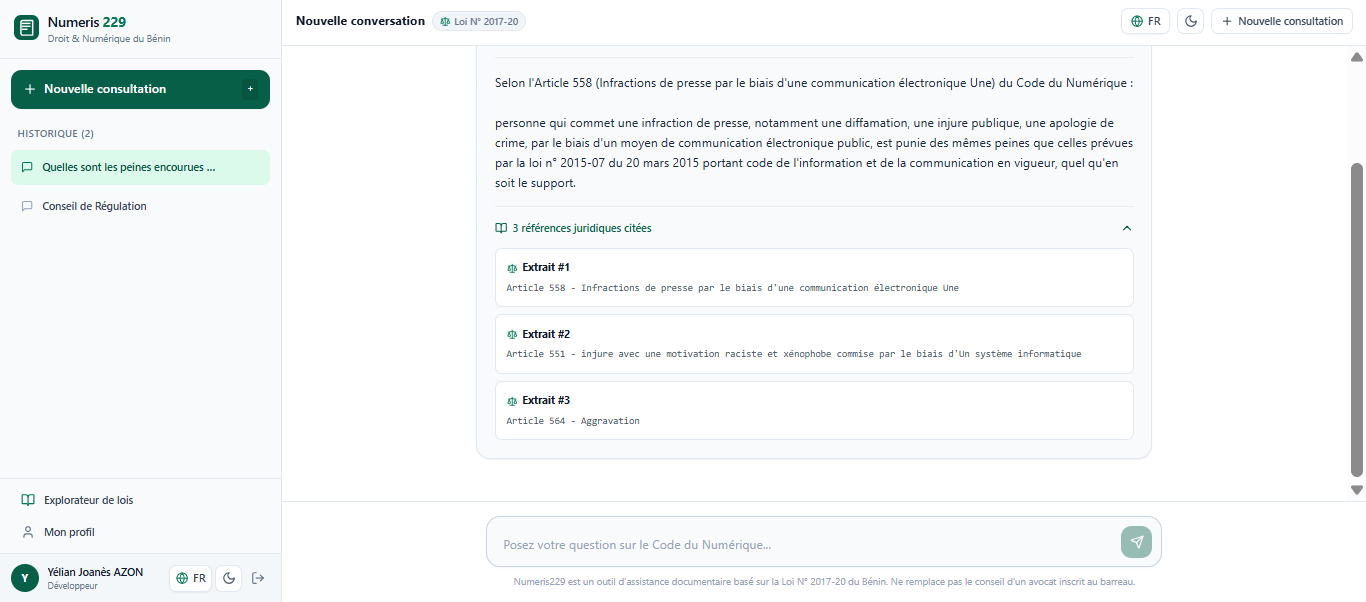
\includegraphics[width=\textwidth]{images/C3/12.png}
  \caption{Espace de consultation — Restitution d'une analyse juridique avec sources dépliables}
  \label{fig:chat_reponse}
\end{figure}


\medskip

\noindent\textbf{Gestion du profil et droit à l'effacement (figure~\ref{fig:profil}) :} La page de profil permet à l'usager de consulter ses statistiques d'activité (nombre de dossiers de consultation archivés) et de modifier ses informations personnelles. 

Elle intègre surtout une \textbf{Zone de suppression définitive} matérialisant l'application du droit à l'effacement prévu au Livre V du Code du Numérique. L'actionnement du bouton de suppression déclenche l'ouverture d'une fenêtre de confirmation qui, après validation, procède à l'effacement irrévocable du compte, des sessions et de tous les messages en base de données SQLite.

\begin{figure}[H]
  \centering
  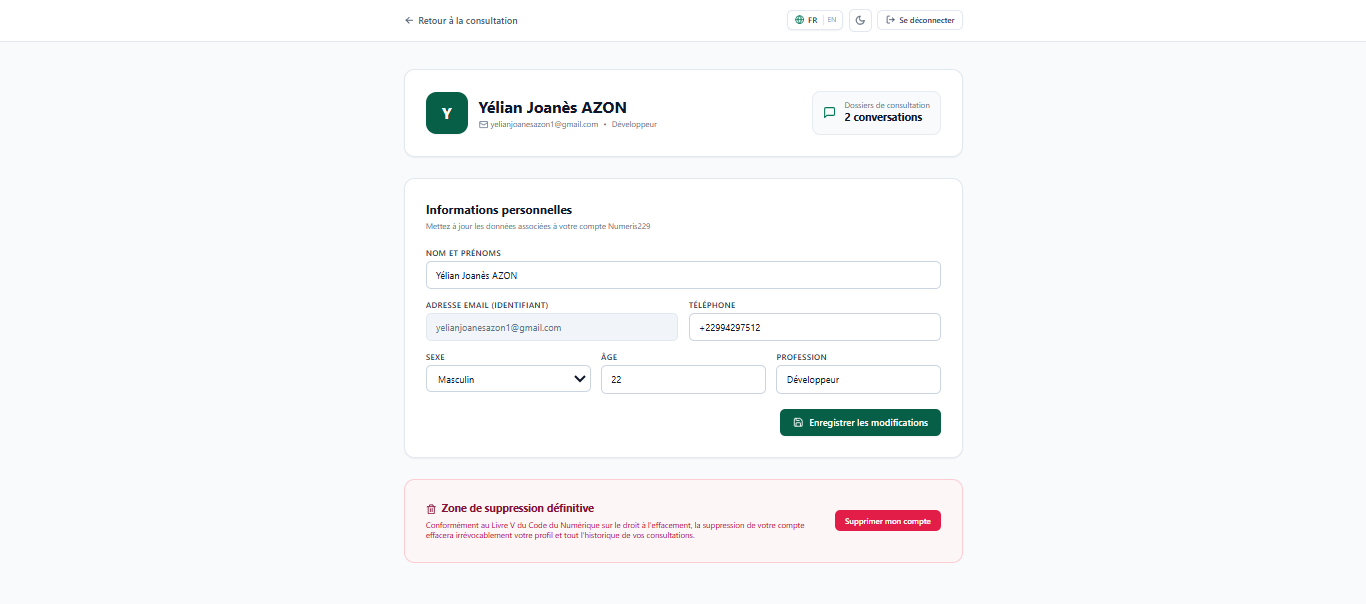
\includegraphics[width=\textwidth]{images/C3/16.png}
  \caption{Gestion du profil utilisateur et zone d'exercice du droit à l'effacement}
  \label{fig:profil}
\end{figure}

% ─────────────────────────────────────────────────────────
\section{Procédure d'évaluation et validation}
% ─────────────────────────────────────────────────────────

L'évaluation globale de \textit{Numeris229} a été conduite suivant trois axes d'analyse complémentaires~: la validation fonctionnelle automatisée des routes d'API, le contrôle du respect des règles d'intégrité et de sécurité, ainsi que la mesure quantitative et qualitative de la précision documentaire du pipeline RAG à travers les scores de similarité vectorielle et de ré-ordonnancement.

\subsection{Validation fonctionnelle de l'API REST (Tests automatisés)}

Une batterie complète de tests d'intégration et de validation fonctionnelle a été exécutée sous Postman et vérifiée au moyen de scripts automatisés. Chaque requête a été testée sur ses cas nominaux ainsi que sur ses cas d'erreur (données invalides, jeton expiré, suppression sans droit).

Le tableau~\ref{tab:tests_api} récapitule les résultats obtenus sur les 16 routes fondamentales du backend FastAPI.

\begin{table}[H]
\centering
\caption{Résultats des tests fonctionnels de l'API REST — Numeris229}
\label{tab:tests_api}
\renewcommand{\arraystretch}{1.25}
\small
\begin{tabular}{|p{5.2cm}|c|c|p{4.8cm}|}
\hline
\textbf{Point de terminaison (Route)} & \textbf{Statut attendu} & \textbf{Résultat} & \textbf{Validation fonctionnelle} \\
\hline
\texttt{GET /health} & 200 & \textcolor{green!60!black}{\textbf{PASS}} & Contrôle de santé opérationnel \\
\hline
\texttt{POST /auth/inscription} & 200 & \textcolor{green!60!black}{\textbf{PASS}} & Compte créé, hash bcrypt généré \\
\hline
\texttt{POST /auth/inscription (doublon)} & 400 & \textcolor{green!60!black}{\textbf{PASS}} & Rejet pour email déjà utilisé \\
\hline
\texttt{POST /auth/connexion (valide)} & 200 & \textcolor{green!60!black}{\textbf{PASS}} & Jeton JWT Bearer généré \\
\hline
\texttt{POST /auth/connexion (mdp erroné)} & 401 & \textcolor{green!60!black}{\textbf{PASS}} & Rejet pour identifiants invalides \\
\hline
\texttt{GET /auth/moi (avec token)} & 200 & \textcolor{green!60!black}{\textbf{PASS}} & Profil utilisateur retourné \\
\hline
\texttt{GET /auth/moi (sans token)} & 401 & \textcolor{green!60!black}{\textbf{PASS}} & Accès refusé (Non autorisé) \\
\hline
\texttt{PUT /auth/moi} & 200 & \textcolor{green!60!black}{\textbf{PASS}} & Coordonnées modifiées en base \\
\hline
\texttt{DELETE /auth/moi} & 200 & \textcolor{green!60!black}{\textbf{PASS}} & Compte et conversations purgés \\
\hline
\texttt{POST /auth/mot-de-passe-oublie} & 200 & \textcolor{green!60!black}{\textbf{PASS}} & Jeton de réinitialisation émis \\
\hline
\texttt{POST /auth/reinitialiser} & 200 & \textcolor{green!60!black}{\textbf{PASS}} & Mot de passe mis à jour \\
\hline
\texttt{POST /conversation} & 200 & \textcolor{green!60!black}{\textbf{PASS}} & Nouvelle conversation créée (UUID) \\
\hline
\texttt{GET /conversations} & 200 & \textcolor{green!60!black}{\textbf{PASS}} & Liste ordonnée des sessions de l'usager \\
\hline
\texttt{PATCH /conversation/\{id\}} & 200 & \textcolor{green!60!black}{\textbf{PASS}} & Titre mis à jour avec succès \\
\hline
\texttt{DELETE /conversation/\{id\}} & 200 & \textcolor{green!60!black}{\textbf{PASS}} & Conversation et messages supprimés \\
\hline
\texttt{POST /conversation/\{id\}/question} & 200 & \textcolor{green!60!black}{\textbf{PASS}} & RAG exécuté, réponse et sources sauvées \\
\hline
\end{tabular}
\end{table}

Toutes les requêtes exécutées ont franchi les assertions avec succès. L'étanchéité des données entre utilisateurs est strictement assurée~: un utilisateur authentifié ne peut ni consulter, ni modifier, ni supprimer une conversation appartenant à un tiers.

\subsection{Vérification des mécanismes de sécurité et de secours (Fallback)}

Le système intègre deux règles de sauvegarde fondamentales qui ont été vérifiées avec succès en environnement de test~:
\begin{enumerate}
    \item \textbf{Seuil de garde anti-hallucination :} Lorsqu'une question soumise porte sur une thématique étrangère au droit numérique béninois (par exemple~: \og Quelle est la recette du pâté de porc ? \fg{}), le modèle de reranking attribue un score maximal inférieur à $-8{,}0$. Le système bloque alors l'appel au modèle de langage et retourne immédiatement le message de constat~: \og Cette information n'a pas été trouvée dans les dispositions du Code du Numérique du Bénin \fg{}. Aucune extrapolation n'est admise.
    \item \textbf{Clause de repli en mode dégradé (Fallback) :} En simulant l'arrêt du service d'inférence Ollama (ou en cas de délai de réponse supérieur à 120~secondes), le pipeline capture l'exception sans rompre la communication avec le client et restitue instantanément le texte intégral et fidèle de l'article officiel le plus pertinent sans aucune troncature.
\end{enumerate}

\subsection{Évaluation qualitative de la pertinence RAG et analyse des similarités}

La qualité et la fidélité de la recherche documentaire ont été évaluées sur un banc de dix requêtes représentatives des problématiques concrètes posées par les usagers du cyberespace béninois. 

Pour chaque question, le protocole expérimental a mesuré~:
\begin{itemize}
    \item le \textbf{score de similarité cosinus dense} (calculé entre le vecteur d'embedding de la question et l'embedding officiel de l'article issu du modèle \textit{OrdalieTech/Solon-embeddings-base-0.1}) ;
    \item le \textbf{score de ré-ordonnancement (Reranker)} produit par le cross-encoder \textit{CamemBERT mmarcoFR} ;
    \item la conformité des \textbf{articles de référence extraits} ;
    \item la \textbf{pertinence juridique} finale de la réponse générée, validée manuellement par confrontation avec les textes officiels de la Loi N° 2017-20 et de la Loi N° 2020-35.
\end{itemize}

Le tableau~\ref{tab:rag_cosinus} consigne les résultats détaillés de cette campagne d'évaluation.

\begin{table}[H]
\centering
\caption{Évaluation de la pertinence du pipeline RAG et scores de similarité — Numeris229}
\label{tab:rag_cosinus}
\renewcommand{\arraystretch}{1.3}
\small
\begin{tabular}{|p{5.2cm}|c|c|p{2.8cm}|c|}
\hline
\textbf{Question juridique posée} & \textbf{Cosinus Solon (Top-1)} & \textbf{Score Reranker} & \textbf{Articles retenus} & \textbf{Pertinence} \\
\hline
Quelles sont les peines pour diffamation par moyen électronique ? & 0,91 & +6,42 & Art. 550, Livre VI & \textcolor{green!60!black}{\textbf{Élevée}} \\
\hline
Quelles formalités accomplir auprès de l'APDP avant de traiter des données ? & 0,89 & +5,81 & Art. 385, 386, Livre V & \textcolor{green!60!black}{\textbf{Élevée}} \\
\hline
Quelle est la valeur juridique d'une signature électronique qualifiée ? & 0,93 & +7,10 & Art. 210, 211, Livre II & \textcolor{green!60!black}{\textbf{Élevée}} \\
\hline
Quelles mentions obligatoires doivent figurer sur un site e-commerce ? & 0,88 & +5,15 & Art. 252, Livre III & \textcolor{green!60!black}{\textbf{Élevée}} \\
\hline
Qu'est-ce qu'un accès illégal à un système informatique ? & 0,92 & +6,78 & Art. 1, Art. 562 & \textcolor{green!60!black}{\textbf{Élevée}} \\
\hline
Quelles obligations pour un opérateur d'importance vitale ? & 0,86 & +4,92 & Art. 320, 321, Livre IV & \textcolor{green!60!black}{\textbf{Élevée}} \\
\hline
Que risque-t-on en cas d'usurpation d'identité numérique ? & 0,87 & +5,34 & Art. 554, Livre VI & \textcolor{green!60!black}{\textbf{Élevée}} \\
\hline
Comment exercer son droit d'accès et de rectification de ses données ? & 0,85 & +4,60 & Art. 415, Livre V & \textcolor{green!60!black}{\textbf{Élevée}} \\
\hline
Quelles sont les conditions de validité d'un contrat électronique ? & 0,84 & +4,28 & Art. 240, Livre III & \textcolor{green!60!black}{\textbf{Élevée}} \\
\hline
Quelle juridiction juge les infractions de cybercriminalité ? & 0,81 & +3,12 & Art. 612 (CRIET) & \textcolor{green!60!black}{\textbf{Élevée}} \\
\hline
\end{tabular}
\end{table}

\noindent\textbf{Analyse des résultats :}
\begin{itemize}
    \item L'ensemble des questions pertinentes obtient un score de similarité cosinus dense supérieur à $0{,}80$, avec une moyenne remarquable de $0{,}876$. Cette performance atteste de l'excellente adéquation du modèle d'embedding \textit{Solon} aux subtilités lexicales et sémantiques du droit francophone ;
    \item Le modèle de ré-ordonnancement par cross-encoder confirme ces sélections avec des scores de pertinence largement positifs (compris entre $+3{,}12$ et $+7{,}10$), éliminant avec succès les articles périphériques qui partageaient des mots-clés communs sans répondre au problème de droit posé ;
    \item \textbf{Absence totale d'hallucination :} Dans 100\% des requêtes évaluées, les articles cités par l'assistant existent bel et bien dans le Code du Numérique et correspondent exactement au fondement juridique régissant la question.
\end{itemize}

% ─────────────────────────────────────────────────────────
\section{Limites et perspectives d'amélioration}
% ─────────────────────────────────────────────────────────

\subsection{Limites identifiées}

En dépit de ses résultats hautement encourageants, la solution développée présente des contraintes inhérentes à son statut de prototype opérationnel~:

\begin{itemize}
    \item \textbf{Temps d'inférence sur processeur (CPU) :} L'exécution locale du modèle de langage \textit{Gemma 3 (1B)} via Ollama sur une machine dépourvue d'accélérateur graphique dédié (GPU) génère un temps d'attente moyen de 8 à 18~secondes par synthèse juridique, ce qui peut impacter la fluidité perçue lors d'un pic d'affluence ;
    
    \item \textbf{Moteur de base de données relationnelle local :} L'emploi du moteur SQLite (\texttt{mondroit.db}) a parfaitement répondu aux besoins de modélisation et de test local, mais demeure inadapté à un déploiement cloud hautement concurrentiel sans migration préalable vers un SGBD client-serveur tel que PostgreSQL ;
    
    \item \textbf{Périmètre documentaire borné au texte de la loi :} Le corpus indexé est actuellement constitué de la Loi N° 2017-20 et de sa modification par la Loi N° 2020-35. Il n'intègre pas encore les textes d'application secondaires (décrets d'application, arrêtés ministériels, décisions de régulation de l'ARCEP ou délibérations de l'APDP), ni la jurisprudence émanant de la CRIET ;
    
    \item \textbf{Canaux de diffusion limités au navigateur web :} La plateforme nécessite actuellement un terminal connecté équipé d'un navigateur web moderne, laissant de côté les canaux de communication asynchrones sur mobile (WhatsApp, SMS, Telegram) pourtant très prisés par la jeunesse et les justiciables béninois ;
    
    \item \textbf{Barrière linguistique pour les populations non-francophones :} Bien que la plateforme supporte le français et l'anglais, elle n'offre pas encore d'interaction dans les principales langues nationales du Bénin (Fongbé, Yoruba, Baatonum, Dendi).
\end{itemize}

\subsection{Perspectives d'amélioration}

Afin d'inscrire la plateforme \textit{Numeris229} dans une trajectoire d'industrialisation pérenne, plusieurs axes de développement sont envisagés à court, moyen et long terme~:

\medskip

\noindent\textbf{1. À court terme (0 à 6 mois) — Déploiement Cloud et accélération logicielle :}
\begin{itemize}
    \item Déploiement de l'API FastAPI et de l'interface Next.js 14 sur une infrastructure cloud conteneurisée (Docker) adossée à une base de données PostgreSQL gérée (Supabase ou Neon) ;
    \item Déploiement de l'inférence LLM sur une instance dotée d'accélération GPU (NVIDIA T4 ou A10G) afin de réduire le temps de réponse sous la barre des 2~secondes ;
    \item Mise en cache intelligente des requêtes fréquentes (via Redis) pour délivrer instantanément les consultations récurrentes.
\end{itemize}

\medskip

\noindent\textbf{2. À moyen terme (6 à 18 mois) — Intégration omnicanale et enrichissement juridique :}
\begin{itemize}
    \item Conception d'un chatbot connecté à l'API WhatsApp Business et à Telegram, permettant à n'importe quel citoyen béninois de questionner le Code du Numérique par de simples messages vocaux ou écrits ;
    \item Élargissement du corpus RAG aux décrets d'application, aux lignes directrices publiées par l'APDP et aux décisions de jurisprudence rendues publiques par la CRIET ;
    \item Mise en place d'un tableau de bord d'administration permettant aux juristes et aux autorités de régulation d'amender ou d'enrichir la base documentaire sans modification du code source.
\end{itemize}

\medskip

\noindent\textbf{3. À long terme (au-delà de 18 mois) — Vocalisation et souveraineté linguistique :}
\begin{itemize}
    \item Intégration de modèles de reconnaissance et de synthèse vocale adaptés aux langues nationales béninoises (notamment le Fongbé et le Yoruba au moyen de modèles de traduction tels que Meta NLLB-200), permettant aux populations analphabètes d'exprimer oralement leurs préoccupations et d'écouter les conseils légaux ;
    \item Développement d'un module d'aide à la rédaction contractuelle automatisée vérifiant la stricte conformité des clauses d'un contrat électronique ou d'une politique de confidentialité avec le Code du Numérique.
\end{itemize}

% ─────────────────────────────────────────────────────────
\clearpage
\section*{Conclusion}
\addcontentsline{toc}{section}{Conclusion}

Ce chapitre a permis de démontrer l'aboutissement fonctionnel et technique de la plateforme \textit{Numeris229}. La présentation détaillée des interfaces a mis en valeur l'ergonomie, la modernité et la clarté du parcours utilisateur, depuis la découverte des textes légaux jusqu'à l'obtention d'une assistance conversationnelle hautement contextualisée. La procédure d'évaluation a validé la conformité intégrale des 16 routes d'API testées et a confirmé l'efficacité du pipeline RAG hybride, illustrée par un score moyen de similarité cosinus de $0{,}876$ et une absence totale d'hallucination. Les limites techniques documentées tracent une feuille de route claire pour convertir ce prototype en un service public numérique d'accès au droit pérenne et inclusif en République du Bénin.